\documentclass[paper=A4,abstracton,twoside,openright,11pt,headsepline,BCOR=1cm,DIV=10,utf8]{scrreprt}

% do this first, since title of thesis might contain umlauts
\usepackage[utf8]{inputenc}

% TODO: fill in the information
\newcommand{\englishtitle}{Development of a framework for automated architecture validation}
\newcommand{\germantitle}{Entwicklung eines Frameworks für die Automatisierte Architekturvalidierung}
\newcommand{\authorprename}{Rushanth}
\newcommand{\authorsurname}{Rasaratnam}
\newcommand{\matriculationnumber}{367117}
\newcommand{\examinors}{
	% Prüfer
	Prof. Dr.-Ing. Stefan Kowalewski\\
	Prof. Dr.\,rer.\,nat. Bernhard Rumpe
}
\newcommand{\advisors}{
	% Betreuer
	David Klüner M.Sc. \\
}


% import the preamble (manages all other imported packages)
% TODO: enable/disable specifics for theses written in german
% TODO: enable/disable BA (bachelor thesis) as thesis type
\usepackage[DE=true, BA=true]{preamble}

% Note: if you switch between different languages after the file has been compiled, it might be necessary to create the pdf multiple times to get rid of errors indicating that you havent loaded the package ngerman yet

% !TEX root = ../main.tex

% this file is read before \begin{document}

\DeclareMathOperator{\u8}{u8}
\DeclareMathOperator{\msb}{msb}    % import commands from file

%Abkürzungen:
%Abkürzungen:
\newacronym{i11}{I11}{Lehrstuhl Informatik 11}
\newacronym{RWTH}{RWTH}{Rheinisch-Westfälische Technische Hochschule Aachen}

%Symbole:
%Symbole
\newglossaryentry{symbol:V}{
	name=\ensuremath{V},
	description={Volumen [l]},
	sort=symbolV,type=symbolslist,
}
\newglossaryentry{symbol:pi}{
	name=\ensuremath{\pi},
	description={Kreiszahl [einheitenlos]},
	sort=symbolpi,type=symbolslist,
}

% --------------------------------------preambles-end-----------------------------------------

% Begin of the actual document
\begin{document}
\pagenumbering{Roman}
%\input{tex/commands2.tex}

% User specific options how latex shall split words at the end of a text line
% in case there is not enough space to fit the word. The listed word will be 
% split at the positions marked with -
% The list of words to split 
\hyphenation{
Byte-array
Si-mu-la-tion
Con-straint Con-straints Compare-Con-straints Bit-Mask-Con-straints
}

\pagestyle{scrheadings}

% do not modify the titlepage!
%% !TEX root = ../main.tex
% adapts automatically according to the selected language (for the preamble)
\titlehead{

\begin{textblock}{120}(85,0)
	
\includegraphics[height=3.1cm]{i11_Vector_RGB.pdf}
\end{textblock}
}

\ifthenelse{\boolean{ba}}{
	\newcommand{\thesistypeen}{Bachelor~Thesis}
	\newcommand{\thesistypede}{Bachelorarbeit}
	}{
	\newcommand{\thesistypeen}{Master~Thesis}
	\newcommand{\thesistypede}{Masterarbeit}
	}

  
\ifthenelse{\boolean{german}}{
	\subject{\thesistypede\\ 
	\vspace{0.15cm}\Large{\thesistypeen
	}}
}{
	\subject{\thesistypeen\\ 
	\vspace{0.15 cm}\Large{\thesistypede
	}}
}

\title{
\ifthenelse{\boolean{german}}{\germantitle}{\englishtitle}\\
\vspace{0.25cm}\vfil\Large{
\ifthenelse{\boolean{german}}{\englishtitle}{\germantitle}}
}
\author{\authorname\\
Matrikelnummer: \matriculationnumber}

\publishers{
\ifthenelse{\boolean{german}}{Gutachter}{Examiners}%
:\\ %research mentor
\examinors \\
\vspace{0.25cm}
\vfil
\vfil
\ifthenelse{\boolean{german}}{Betreuer}{Advisors}%
:\\
\advisors

\vfil
\vfil
\vspace{0.25cm}

\ifthenelse{\boolean{german}}{Diese Arbeit wurde vorgelegt am \\Lehrstuhl Informatik 11 -- Embedded Software}{This thesis was submitted to \\Lehrstuhl Informatik 11 -- Embedded Software}
}

\date{ Aachen, \today}



% dynamically set the thesis type according to the used language
\ifthenelse{\boolean{ba}}{
	\newcommand{\thesistypeen}{Bachelor~Thesis}
	\newcommand{\thesistypede}{Bachelorarbeit}
}{
\newcommand{\thesistypeen}{Master~Thesis}
\newcommand{\thesistypede}{Masterarbeit}
}

\ifthenelse{\boolean{german}}{

	\renewcommand{\subject}{\thesistypede\\ 
		\vspace{0.3cm}{\thesistypeen\\}}
	}{
	\renewcommand{\subject}{\thesistypeen\\ 
		\vspace{0.3 cm}{\thesistypede\\}}
	}

% set title page
\renewcommand*{\maketitle}{%
  \begin{titlepage}
  	\begin{textblock}{120}(85,0)
  		
\includegraphics[height=3.1cm]{i11_Vector_RGB.pdf}
  	\end{textblock}
  	
  	% empty
  	\ 
  	\vspace{0.5cm}

	% thesis type
	\centering
	\textbf{\subject}
	
	\vspace{0.8cm}
	\vfill
	
	% thesis title		% TODO: größer & andere Schriftart
	\textbf{
	  \LARGE{\ifthenelse{\boolean{german}}{\germantitle}{\englishtitle}}\\
	  \vspace{0.3cm}
	  \Large{\ifthenelse{\boolean{german}}{\englishtitle}{\germantitle}}\\
    }
  
  	\vspace{0.8cm}
  	\vfill
  	
  	% student
  	\authorname\\
  	Matrikelnummer: \matriculationnumber\\
  	
  	\vspace{0.3cm}
  	\vfill
  	
  	% metainfo
  	Aachen, \today
  	\vspace{0.3cm}
  	\vfill
  	 
  	\ifthenelse{\boolean{german}}{Gutachter}{Examiners}%
  	:\\ %research mentor
  	\examinors \\
  	\vspace{0.3cm}
  	\vfil
  	\ifthenelse{\boolean{german}}{Betreuer}{Advisors}%
  	:\\
  	\advisors
  	
    \vspace{0.3cm}
    \vfill
    	
    \ifthenelse{\boolean{german}}{Diese Arbeit wurde vorgelegt am \\Lehrstuhl Informatik 11 -- Embedded Software}{This thesis was submitted to \\Lehrstuhl Informatik 11 -- Embedded Software}
  
  	
   
  \end{titlepage}
}

\maketitle

% OPTIONAL (remove if you don't want a dedication)
% define basic appearence for dedication
\renewcommand{\dedication}{
	\cleardoublepage
	\thispagestyle{plain}
	\ \par
	\vspace{5cm}
	\noindent
	\ifthenelse{\boolean{german}}{\textbf{Dankeswort}}{\textbf{Acknowledgments}}
	\vspace{-0.5cm}
	\begin{flushleft}
		\noindent
	\end{flushleft}}

\dedication{
\ifthenelse{\boolean{german}}{
Vorab möchte ich mich bei einigen Personen bedanken, die mich bei der Erstellung dieser Arbeit unterstützt haben:
}{
Ex ante, I'd like to thank the listed persons below who supported me during the editing time of this thesis:
}
\begin{itemize}
	\item Person XY for ...,
	\item The coffee machine of i11.
\end{itemize}
}

\listoftodos[This is to be done] 	% TODO: exclude in final version
% the list of todos should not be part of the final thesis and is only intended to show the advisor(s) of what flaws the student is already aware of)

% Abstract of the thesis
% !TEX root = ../main.tex
\begin{abstract}

% Für deutschsprachige Ausarbeitungen sollte jeweils ein Abstract in deutscher und englischer Sprache verfasst werden
% If written in german their should be two, a german and an english abstract


% Kurze Motivation und Angabe was in der Arbeit behandelt wird. Dies wird in der Einleitung ausführlicher behandelt.
% Brief motivation and explanation of the topic. This will typically be repeated more extensive in the "`introduction"' chapter.
\noindent
An abstract is basically a very short summary of the thesis topic.
It describes short and precise the content of the thesis and what has been achieved.
An abstract should not contain any discussion, quotation or reference to figures, chapters and so on.
Please note that if you write your thesis in german, there should be a german and english version of the abstract.
Although an abstract should generally not contain examples we provide here an example abstract for this document:\\

% Beispiel eines Abstracts für dieses Dokument
% Example of an abstract for this document
There exists a large variety of latex templates such as guidelines explaining or demonstrating the common structuring, dos and donts of bachelor and master theses.
This document aims at providing an example for a typical structure of such theses containing useful knowledge about scientific writing and providing students with a correspondent latex template for bachelor or master theses at i11.
Moreover, it gives some advice on very basic latex functionality for citation and figure handling.


\end{abstract}


% Eidesstattliche Erklärung
% Note: there is an english translation available (eidesstattlicheVersicherungZPA_en.pdf). 
% However, the german version is legally binding and required to be a part of the thesis.
%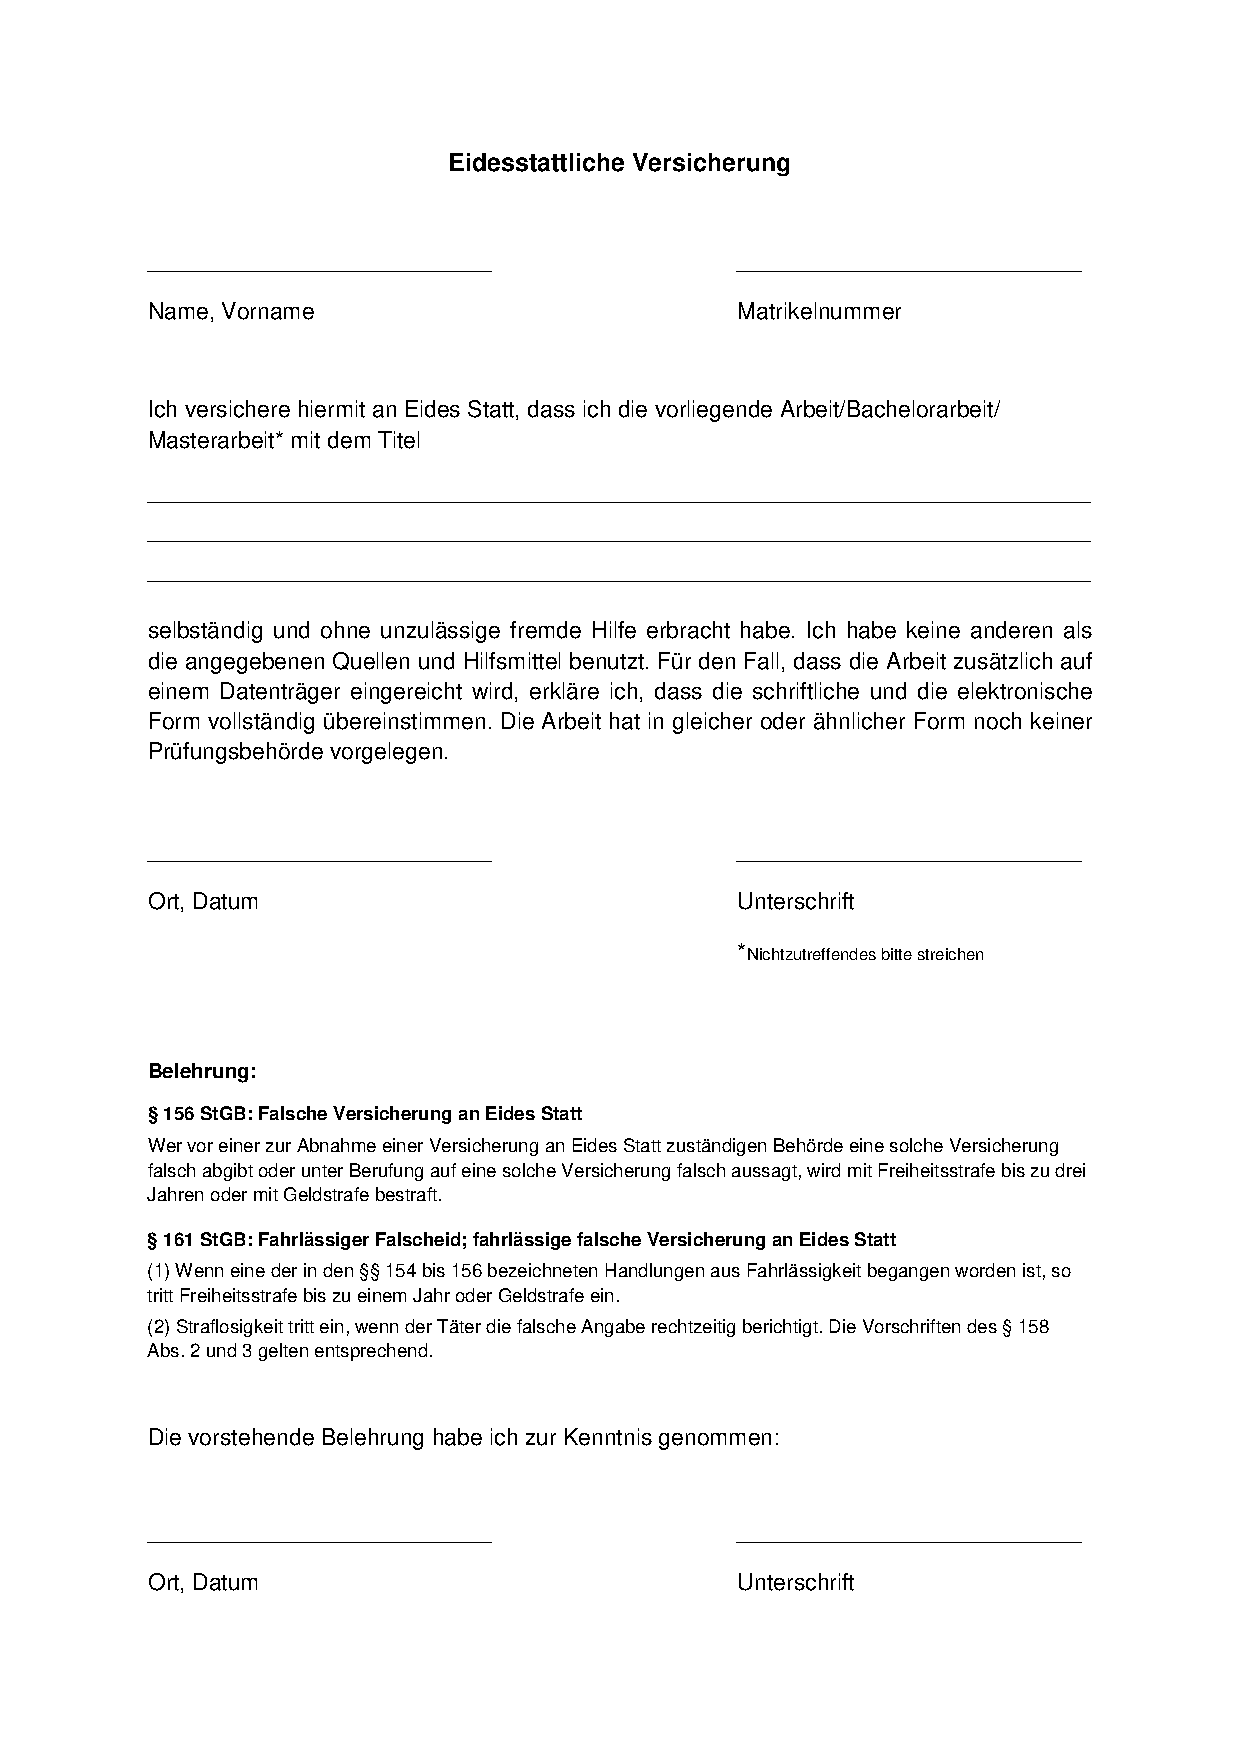
\includepdf[pages={1}]{eidesstattlicheVersicherungZPA.pdf}
% this page may not be manipulated

\newpage
\thispagestyle{empty}
\begin{center}
	\Large\textbf{Eidesstattliche Versicherung}
\end{center}
\vspace{5mm}

\begin{spacing}{0.4}
\noindent 
\begin{minipage}[t]{0.41\textwidth}
		\authorsurname,~\authorprename\\
		\noindent 
		\rule{\textwidth}{0.4pt} \\\\
		Name, Vorname
\end{minipage}
\hfill
\begin{minipage}[t]{0.41\textwidth}
	\matriculationnumber\\
	\noindent 
	\rule{\textwidth}{0.4pt}\\\\
	Matrikelnummer
\end{minipage}
\end{spacing}


\vspace{10mm}
\noindent
Ich versichere hiermit an Eides Statt, dass ich die vorliegende \ifthenelse{\boolean{ba}}{Bachelorarbeit}{Masterarbeit} mit dem Titel
\vspace{4mm}

\noindent
\textbf{\germantitle}


\vspace{4mm}
\noindent
selbständig und ohne unzulässige fremde Hilfe erbracht habe. Ich habe keine anderen als die angegebenen Quellen und Hilfsmittel benutzt. Für den Fall, dass die Arbeit zusätzlich auf einem Datenträger eingereicht wird, erkläre ich, dass die schriftliche und die elektronische Form vollständig übereinstimmen. Die Arbeit hat in gleicher oder ähnlicher Form noch keiner Prüfungsbehörde vorgelegen.\\
\vspace{4mm}
\vfil

\begin{spacing}{0.4}
\noindent 
\begin{minipage}[t]{0.41\textwidth}
	\rule{\textwidth}{0.4pt}\\\\
	Ort, Datum
\end{minipage}
\hfill
\begin{minipage}[t]{0.41\textwidth}
	\rule{\textwidth}{0.4pt}\\\\
	Unterschrift
\end{minipage}
\end{spacing}

\vfill
%\vspace{14mm}
\noindent
\textbf{Belehrung:}

\vspace{4mm}
\vfil
\noindent
\textbf{\S~156 StGB: Falsche Versicherung an Eides Statt}\\
Wer vor einer zur Abnahme einer Versicherung an Eides Statt zuständigen Behörde eine solche Versicherung
falsch abgibt oder unter Berufung auf eine solche Versicherung falsch aussagt, wird mit Freiheitsstrafe bis zu drei
Jahren oder mit Geldstrafe bestraft.\\


\noindent
\textbf{\S~161 StGB: Fahrlässiger Falscheid; fahrlässige falsche Versicherung an Eides Statt}\\
(1) Wenn eine der in den §§ 154 bis 156 bezeichneten Handlungen aus Fahrlässigkeit begangen worden ist, so
tritt Freiheitsstrafe bis zu einem Jahr oder Geldstrafe ein.\\
(2) Straflosigkeit tritt ein, wenn der Täter die falsche Angabe rechtzeitig berichtigt. Die Vorschriften des § 158
Abs. 2 und 3 gelten entsprechend.\\


\noindent
\normalsize Die vorstehende Belehrung habe ich zur Kenntnis genommen:\\
\vspace{4mm}
\vfil

\begin{spacing}{0.4}
	\noindent 
	\begin{minipage}[t]{0.41\textwidth}
		\rule{\textwidth}{0.4pt}\\\\
		Ort, Datum
	\end{minipage}
	\hfill
	\begin{minipage}[t]{0.41\textwidth}
		\rule{\textwidth}{0.4pt}\\\\
		Unterschrift
	\end{minipage}
\end{spacing}


% TODO: remove/add % symbols before the required rows
\tableofcontents  % Inhaltsverzeichnis
\listoftables		% Tabellenverzeichnis
\listoffigures   % Abbildungsverzeichnis

% TODO: see http://texblog.org/2014/01/15/glossary-and-list-of-acronyms-with-latex/ 
% at Capitalize and pluralize terms for a brief introduction on how to use acronyms 

% print acronym list
\ifthenelse{\boolean{german}}{
	\printglossary[type=\acronymtype,style=long, title=Abkürzungsverzeichnis] % use this for german version
}{
	\printglossary[type=\acronymtype,style=long, title=List of Acronyms]
}

% print symbol list
\ifthenelse{\boolean{german}}{
	\printglossary[type=symbolslist,style=long, title=Symbolverzeichnis] % use this for german version
}{
	\printglossary[type=symbolslist,style=long, title=List of Symbols]
}

\pagestyle{scrheadings}

% TODO: write your content into the chapters
\cleardoublepage\pagenumbering{arabic}
% !TEX root = ../main.tex

%\chapter{Einleitung}
\chapter{Introduction}
\label{sect:introduction}

% Thema motivieren, worum geht es und warum ist das wichtig?
% Motivate the topic, what is this thesis about and why is that important?

An introduction motivates the topic of the thesis and explains the origin of the task. \todo{Motivate the topic, what is this thesis about and why is that important?}
It starts often with a very general statement followed by explanations which difficulties (of course with relevance to the thesis topic) arise.
Finally, the difficulties are narrowed down to the topic of the thesis.
At this point the reader should understand the relevance of the problem being addressed by the thesis.
An example for an introduction could look like the text following below. \\

At the end of their bachelor or master studies young students have to write a final thesis.
For many of them this is their first written academic document of mentionable relevance.
Thus, those students have no experience with academic writing and therefore require often some basic guidelines.
Guidelines are usually provided directly by the thesis advisers up front and/or during thesis review.
Providing such guidelines in a written and structured form to the students results hopefully in less review work for advisor and student, more consistent and clear theses and hence theses of better quality. \todo{Dies ist eine Anmerkung was noch zu machen ist.}

%\section{Aufgabenstellung}
section{Main contributions}
\label{sect:main_contributions}
% Was soll gemacht werden?
% What shall be done within this thesis
This document aims at providing a basic template for students writing their bachelor or master thesis at \abk{i11}.
It shall provide a basic overview on how such writings are structured and provide some useful hints.

%\section{Gliederung}
\section{Outline}

% Wie ist die Arbeit aufgebaut? Dies sollte den roten Faden beschreiben der sich durch die ganze Arbeit zieht und den Zusammenhang der einzelnen Teile verdeutlichen.
% How is this document structured? 

The outline of a thesis should point out how the different chapters are related to each other and that the thesis is well structured.
It should show that the different chapters form a single coherent document.
An example how such an outline could look like for this document is given below.\\

Chapter~\ref{sect:basics} gives an introduction and overview on latex citations and figures to provide some basic knowledge how to handle those latex-constructs.
The proximate Chap.~\ref{sect:relatedWork} presents an overview of work related to this document.
Chapter~\ref{sect:corechapter} introduces subsequently how citations have to be used in order to avoid wrong citation styles or even plagiarism.
It therefore requires information introduced before in chapter \ref{sect:basics}.
Additionally, this chapter provides some hints dealing with figures in latex and their quality.
The document is concluded by Chap.~\ref{sect:conclusion} which gives also an outlook how this document could be extended in the future.

% !TEX root = ../main.tex
\chapter{Background}
%\chapter{Grundlagen}
\label{sect:basics}

The chapter about the background should introduce all preliminary knowledge the reader should have before reading the part of the thesis where the actual contribution to a topic is presented.
Such preliminary knowledge could be theoretic aspects, domain knowledge or special notations being used, e.\,g., diagram types for visualization purpose.
Generally this chapter does not present any contributions of the author.
Thus, the background chapter makes often extensive use of citations providing the information whose work is presented.
In case the background chapter presents nonetheless work of the thesis author, make sure that this is absolutely clear.

% Jedes Kapitel/Abschnitt sollte mit einem (zumindest kurzen) einführenden Text beginnen der 
% erklärt worum es in diesem Kapitel geht (siehe About Chapters and Sections)
% Each chapter should start with an (short) introduction explaining what the chapter is about 
% (see About Chapters and Sections)



% Die Abschnitte des Grundlagenkapitels sind exemplarisch!
% The sections of the fundamentals chapter are only examples!



\section{About Chapters and Sections}
\label{sect:chaptsect}

At the beginning of each chapter or section the writer should introduce the reader to the specific (sub-)topic addressed.
This is intended to provide a continuous reading experience.
In a similar way, there should be some final words at the end of each chapter or section anticipating the next subtopic.
Of course, the chapters and sections have to be ordered such that there is a connection between them.
An outline about the different sections of a chapter shall be given at the beginning of each chapter, too.
Moreover, please ensure that different headings do not consecutively follow each other without text in between.
After this section has dealt with the connections between different chapters and sections, the next section explains some frequently used latex commands.

An example how this could look like for the beginning of the Background chapter which should have been written before this section is given below:\\
This chapter presents some latex fundamentals and is divided into two sections.
The first section \ref{sect:chaptsect} deals with the structuring of the text, namely introductions and connections between chapters and sections.
The second section \ref{sect:latex} presents some basic knowledge on setting up the latex environment to create this document and two latex commands which will be used.

% ----------------------------------------------------------------------------------------------------

\section{Latex-technicals}
\label{sect:latex}

This section intends to introduce the reader without or only few latex knowledge to some basic latex commands.
It starts with a short introduction on how to get started with Latex and the setup of a latex environment.
In order to explain some useful features for document creation, Sect.~\ref{sect:citations} presents a citation command and gives some instructions on \textit{bibtex}.
Consequently, Sect.~\ref{sect:illustrations} explains how illustrations can be added to a document\footnote{A brief explanation on how to use symbols and abbreviations with this template can be found in appendix \ref{app:c}}.

\subsection{Setting up the environment}
\label{sect:latexenvironment}
The creation of documents using Latex can be compared to the creation of programs using a programming language like C.
This means that the Latex source files are simple text files.
These files describe the document being constructed and can be \enquote{compiled} to generate the document.
Accordingly a latex compiler is required by the user to create documents.
The open source project MiKTeX\footnote{\url{http://miktex.org/about}} includes such compilers.
This software-package contains everything needed to create Latex files out of this template.
Please note, that it does not contain all required packages to compile this document.
However, it is possible to obtain the required packages during latex compilation automatically.
If this is not initially the case, the feature can be enabled by starting the configuration program located at \enquote{Miktex install directory/miktex/bin/x64/mo\_admin}.
The option is configurable under the general tab at the section \enquote{package installation}.
Depending on the enabled/used features (e.\,g., creation of index etc.) this document requires to be created with additional parameters what can easily be done using the \texttt{compile.bat} script, delivered with this template.

As for programming languages \textit{Integrated Development Environments} (IDE) can support the user during his work.
An example for such an IDE compatible with MiKTeX is TeXnicCenter.
The reader might want to take a look at the correspondent website \url{http://www.texniccenter.org/}.


Since it has been explained how a Latex environment can be set up the following two sections describe some basic commands which will be needed to create scientific documents.

\subsection{Citations}
\label{sect:citations}

Latex is widely used to write scientific papers or theses.
A general commonality of such documents is the need to refer to work provided by other parties.
To cope with this need latex provides in combination with bibtex\footnote{bibtex is used to generate the bibliography} the \textbackslash cite\{reference-tag\} command.
During the creation of a latex document occurrences of the \textbackslash cite\{\} command are automatically replaced with squared brackets and a generated tag in between.
Those tags are listed in the bibliography with information about author, publisher, etc. referring to the literature information was taken from.
For instance, the command \textbackslash cite\{columbia\} will be transformed during creation of this latex document into \cite{columbia}.
This transformation requires that there is a correspondent entry for the \enquote{columbia} reference-tag in the \enquote{references.bib} file which comes with this latex template\footnote{In case a web content is referenced, a timestamp indicating the content was consulted shall be part of the bibliography entry. 
Moreover, offline copies of the contents need to be provided. This ensures that readers will be able to understand your work in the future when cited web content may have changed or be unavailable.}.

The next latex feature introduced in this document is the possibility to use illustrations, which is the topic of the following section.

\subsection{Illustrations}
\label{sect:illustrations}

Latex documents may contain pictures to support and visualize explanations.
They can be added to a document using the following commands:

\begin{flushleft}

\textbackslash begin\{figure\} \\
	\textbackslash centering \\
		\textbackslash includegraphics\{path\_to\_picture\} \\
	\textbackslash caption\{This caption will be shown below the figure\} \\
	\textbackslash label\{fig:label\_to\_referrence\_the\_figure\} \\
\textbackslash end\{figure\} \\

\end{flushleft}


An example how this looks after creation of the document is shown in Fig.~\ref{fig:logo}.
\begin{figure}[H]
	\centering
		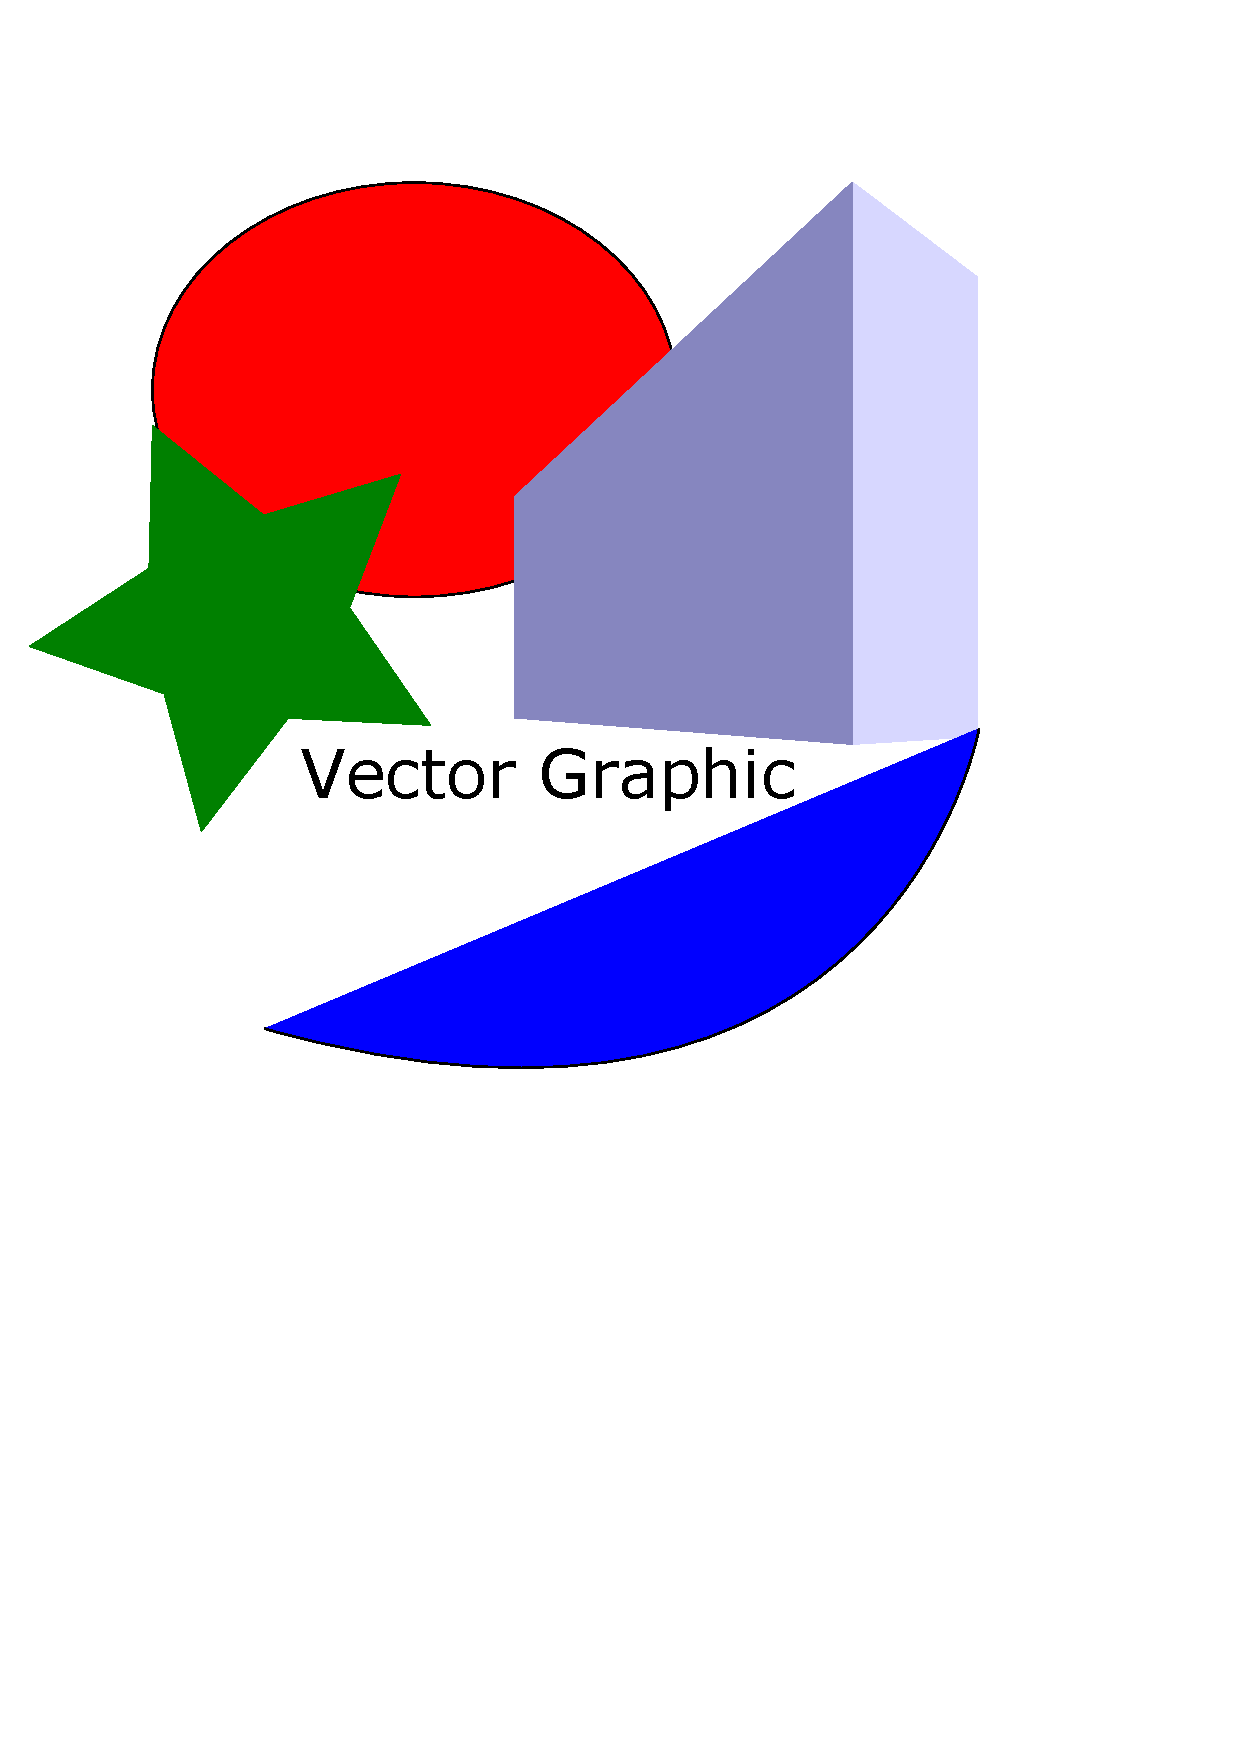
\includegraphics[width=0.40\textwidth]{figures/vectorGraphic.pdf}
	\caption{Example of a vector graphic}
	\label{fig:logo}
\end{figure}

Since this document is not the first and only one providing advice and hints regarding latex and structuring theses, the following chapter presents related work in this field.
% !TEX root = ../main.tex

%\chapter{Verwandte Arbeiten}
\chapter{Related Work}
\label{sect:relatedWork}

% Dieses Kapitel kann auch als Abschnitt im vorherigem Grundlagen Kapitel enthalten sein.
% Dies kann je nach Art der verwandten Arbeit und wie diese mit der aktuellen Arbeit verknüpft ist eine logischere Gliederung darstellen.
% This chapter can alternatively be a section of the background chapter. Depending on the relations between the actual and the related work,
% it can be a more intuitive, logic and consistent structuring to mention the related work in the previous chapter.

% Kurz vorstellen was es noch in dem Gebiet gibt und worin sich diese Arbeit davon unterscheidet
% Short presentation/summary of what has been done already in the research area and how it differs from the current thesis.

Their are many books on other guidelines describing how a bachelor or master thesis should be structured which cannot all be mentioned here.
Hence, this chapter limits its scope to a single example.
For instance the university of columbia provides some guidelines on writing theses \cite{columbia}.
According to the guideline a thesis starts with a title page with information about the title, author, department, delivery date, research mentor(s), advisors, their institutions and email adresses.
The next structuring elements are the table of contents, the list of figures and the list of tables before the introduction of the thesis.

...

The main difference between the described guideline and this document is that the guideline addresses some more questions of methodological nature to be answered.
This document however provides a more specific structure and layout template for theses written with latex at i11 in the field of computer science.
Additionally, this document gives advice on some more practical topics.


% !TEX root = ../main.tex

\chapter{Inhaltsspezifische Überschrift}
%\chapter{Very Specific Title}
\label{sect:corechapter}

% Kernstück der Arbeit (eventuell auch in mehrere Kapitel unterteilt). Hier wird konkret vorgestellt, was entwickelt wurde und wie dies von statten ging.
% This chapter (maybe split in multiple) is the main part of the thesis. It presents what was realized, how things were realized, 

As already stated before in chapter \ref{sect:chaptsect}, every chapter or section should start with some introducing words.
Due to the fact that this chapter (or potentially multiple chapters) presents the authors efforts, each section and chapter shall provide analogous to its introduction some concluding words, summarizing the findings and achievements of the specific section or chapter.


% Alles aus dem Grundlagen-Kapitel kann ohne weitere Erklärung genutzt werden. nicht zu erwarten ist, dass der leser über nicht präsentierte Zusatzinformationen zum Thema verfügt.
% The information presented before in the background chapter can be used without further explanation. However you should not assume that the reader knows further details on the topic which were not presented in this thesis.
\section{Different Citation Types}

During the writing of a thesis work, ideas and contributions provided by other people then the author have to be declared as such.
This is done using citations.
In general, there are two different types of citations.
The first type of citation is the literal citation.
It is only used if text is copied directly without modification from others.
In this case the citation is surrounded by quotes "".
For instance:
\begin{center}
Wikipedia states that \enquote{Wörtliche Zitate sollten eingesetzt werden, wenn nicht nur der Inhalt der Aussage, sondern auch deren Formulierung von Bedeutung ist} \cite{wikicite}.
\end{center}
Nonetheless, the author has to make unambiguously clear where the citation originates from.
In case of the wikipedia citation above this is done with: \cite{wikicite}.


The second citation type is the more frequent used reference using the \textbackslash cite\{\} command presented in Sect.~\ref{sect:citations}.
This citation type is used if no literal citation is used.
For instance:
\begin{center}
If not only the content of a statement is of importance but also the original wording, then literal citation using quotes has to be used \cite{wikicite}.
\end{center}
Such references have to follow directly the first statement taken from other sources.

The following example shows how this looks for bigger paragraphs.
The same colored parts refer to the same source.

\begin{flushleft}
\textcolor[rgb]{1,0,0}{Welche Theorien standardmäßig von einem Programm zur Lösung von SMT-Problemen unterstützt werden hängt vom konkret verwendeten Programm ab \cite{smtappetizer}.
Zur Vereinheitlichung der Beschreibung von Theorien, so wie der Eingabe- und Ausgabesprache für Programme die SMT-Probleme lösen wurde der SMT-LIB Standard verfasst.}
\textcolor[rgb]{0.2,0.8,0.2}{Aktuell befindet sich dieser von der SMT-LIB Initiative formulierte Standard in Version 2.0 \cite{smtlib}.}
\textcolor[rgb]{0,0.8,1}{Zu diesen Theorien gehören die Theorie der Felder (engl. \textit{arrays}), der Bit-Vektoren fester Größe, der booleschen Operatoren, der Fließkommazahlen, der Ganzzahlen, der reellen Zahlen und der Kombination von reellen und ganzen Zahlen \cite{smtlibweb}.}
\end{flushleft}

Please ensure that the visual look of the automatically generated bibliography is consistent and the printed information is complete.
For instance:
\begin{itemize}
	\item the separation of words at the end of a line should be adequate
	\item the ISBN, DOI, etc. are formatted the same way for every bibliography entry
	\item every web-sources accessing-date is stated
	\item URLs are displayed the way they are intended to (e.g. underscores in copied links are interpreted by latex as commands and not displayed unless the url is surrounded by \textbackslash url\{\} or backslashes are interpreted as escaping characters and should be replaced with \textbackslash textbackslash)
\end{itemize}
It is the responsibility of the author of a thesis to ensure that all relevant information about the used literature is readable in the printed version of the thesis.

The next section gives advice on figures used in the document and extends the citation concept accordingly.


\section{Citations and Advice on Illustrations}

Similar to textual content, pictures may originate from other publications, too.
Thus, they have to be declared as results of work from others.
In case the figure is not modified in any way this can be done by adding a correspondent citation in the figures caption.
If the figure has been redrawn or modified the reference can be given as shown below:
\begin{figure}[H]
	\centering
		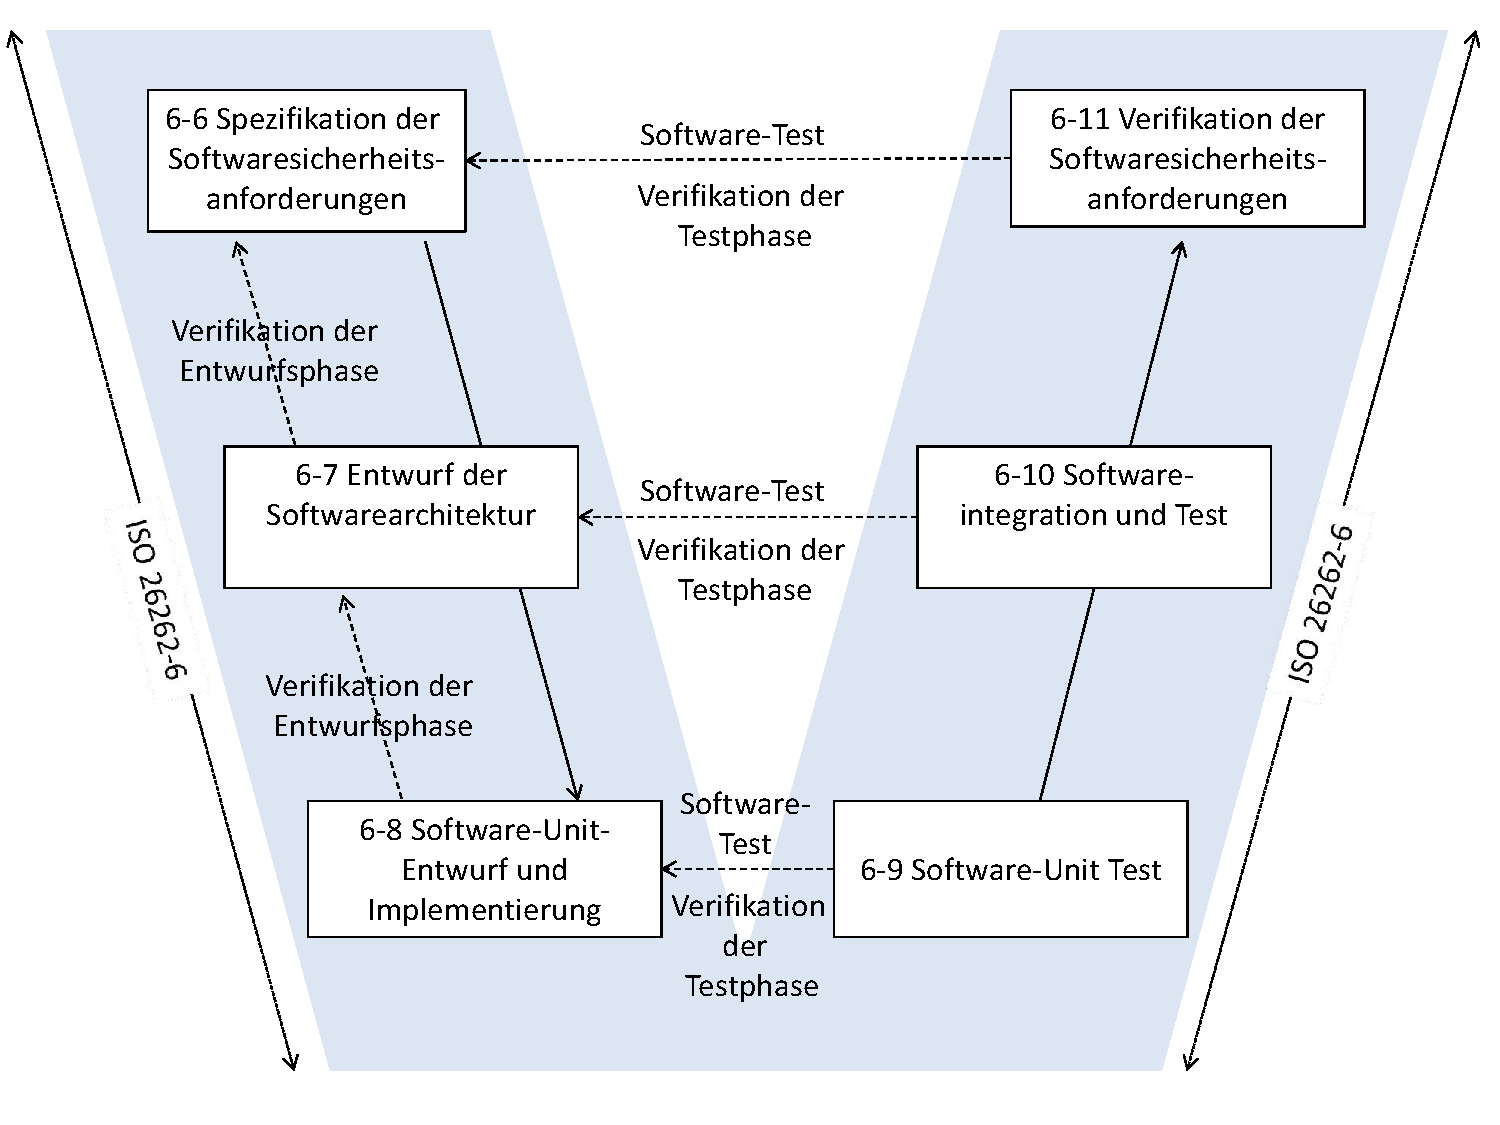
\includegraphics[width=0.80\textwidth]{figures/V-Modell.pdf}
	\caption{V-Modell correspondent to ISO 26262-6 (drawing after \cite{verificationvalidation})}
	\label{fig:vmodell}
\end{figure}

The author might even differentiate between different figure-citation-types.
Those could be:
\begin{itemize}
	\item taken from \textit{(exact copy of the figure)}
	\item partly taken from \textit{(parts of the figure are taken from the specified source, others were added by the author)}
	\item adaption/extension of
	\item redrawing of \textit{(the figure has been redrawn)}
\end{itemize}
If such descriptions or correspondent abbreviations are used the author should specify upfront the semantic and syntax at the beginning of the thesis.
The important thing here is not which words were used but that it is clear which parts are whose work.
\\\\
\textsl{\textcolor[rgb]{0.75,0.75,0.75}{It follows an example for a bad structuring of paragraphs and transition between such since the quality of figures does not relate to figure citations.}}
Also it is not recommendable to use fonts, \textcolor[rgb]{1,1,0}{colors} and other \textsl{\textit{\colorbox[rgb]{1,1,0.6}{\textcolor[rgb]{0.8,1,0.8}{styling}}}} elements (even in figures) which cannot be read easily.
\\\\
Figures should always be provided as vector graphics, e.g. *.svg or *.pdf files.
The benefit of such formats is their scalability without loss of quality.
Unfortunately, many pictures are not provided as such.
Hence, schemata etc. need often to be redrawn.
Some tools supporting the creation of vector graphics are:
\begin{itemize}
	\item inkscape (open source)
	\item powerpoint (create a slide composed of shapes and store it as *.pdf file) or word/excel\\
	(this should work with open office too)
	\item to be completed ...
\end{itemize}
Please note that importing non vector graphics, e.g. bitmaps, by the mentioned tools will not convert them into vector graphics.
Another aspect which should be addressed regarding figures in latex documents is the size of text inside figures.
Due to scale operations on figures (see \ref{fig:vmodell} where the width of the figure is set to 80 percent of the width of the region where text can be shown) the size of text labels in figures may change.
However, the size of the smallest text on a figure should never be smaller than the smallest text-size of the rest of the document.
Moreover the sizes of texts on figures should not change arbitrary between illustrations.

After this part of many theses follows an evaluation.
Some important points regarding the evaluation part are mentioned in the following chapter.

% !TEX root = ../main.tex

\chapter{Evaluation}
\label{sect:evaluation}

Since there is no evaluation for this document, this chapter lists some points which may be considered when evaluating software/algorithms/procedures.
\begin{itemize}
	\item Comparison with other approaches to achieve the same goal as this work
	\item Measure resources needed by a developed tool/procedure/etc. regarding (time consumption, cpu usage, memory usage, ...)
	\item What about the quality of the results?
	\item Are there any problems with the procedure/applicability or restrictions?
	\item Evaluate (if possible) using \enquote{real world examples} and not only academic ones.
\end{itemize}

Please note that they do not all have to apply or be suitable for any thesis topic.
It might be that evaluation results are not presentable in a structured and readable way.
For instance, if tables become to large.
In such cases it might be helpful to place the results in the appendix \ref{app:a} and refer to them.
This applies also for figures, test specifications and tables at any other place in the thesis and is the only exception allowing forward references.
The evaluation should state very clear what is possible and what is not.
If there are any, the limits of the developed approach should be shown using suitable examples.
Do not be afraid to show limitations of approaches.
This does generally not undermine the authors achievement if it is clear and can be explained why the limitations exist.
The author should avoid to use vague words like better, worse, etc. to describe the evaluation results.
This applies in general for the other chapters of the thesis, too.

The next chapter of this document is the final chapter, which should always conclude the work presented before.	% If there is one

% !TEX root = ../main.tex

%\chapter{Fazit}
\chapter{Conclusion}
\label{sect:conclusion}
		
% Gehe auf Ziel, Aufgabenstellung aus Einleitung ein und wiederhole zusammenfassend, wie die Aufgabenstellung erfüllt wurde und was die Ergebnisse sind.
% Adress the aim and the conceptual formulation of the assignment from the introduction directly and summarise how the formulated goals were reached (or not).

The aim of this document was to provide students at the end of their studies with a template for their written thesis.
Due to the common lack of experience in the field of academic writing this work is intended to provide a template for structured writing.
Therefore, this entire document is structured as a thesis should usually be.

Moreover it provides some hints how citations should be used and how figures should be dealt with to achieve high quality versions of latex documents.
In contrary to this sentence, a conclusion should not introduce new information, about the topics discussed before, which has not yet been presented.

The following (optional) section provides some further ideas for potential extension of this work.

%\section{Ausblick} %(optional)
\section{Future Work} % (optional)

% Wie könnte es weiter gehen? Dieser Abschnitt kann auch in einem eigenen Kapitel vorhergehen.
% Short description how this work could be pursued. This can be done in a separate chapter preceding the conclusion, too.

There are many possible ways how this short document could be extended in the future.
One may think of additional explanations regarding latex and its use, with the extend to an entire latex tutorial.
A further extension could be the definition of helpful latex commands or a documentation on commonly used latex commands and packages.

\bibliographystyle{alphadin}
\bibliography{references}

\appendix	%TODO: (optional)
% !TEX root = ../main.tex

\chapter{Appendix1}
\label{app:a}

Here could be a large figure or a very big table like this:

\begin{tabularx}{\textwidth}{| p{0.2\textwidth} | p{0.4\textwidth} | p{0.2\textwidth} |}%{\linewidth}{|X|X|}
  \caption{Table caption} \\\endfirsthead
	
  \hline
  \textbf{column1} & column2 & column3 \\ \hline
  row 1 & X & X \\ \hline
	row 2 & X & X \\ \hline
	row 3 & X & X \\ \hline
	row 4 & X & X \\ \hline
	row 5 & X & X \\ \hline
	row 6 & X & X \\ \hline
	row 7 & X & X \\ \hline
	row 8 & X & X \\ \hline
	row 9 & X & X \\ \hline
	row 10 & X & X \\ \hline
	row 11 & X & X \\ \hline
	row 12& X & X \\ \hline
	row 13 & X & X \\ \hline
	row 14 & X & X \\ \hline
	row 15 & X & X \\ \hline
	row 16 & X & X \\ \hline
	row 17 & X & X \\ \hline
	row 18 & X & X \\ \hline
	row 19 & X & X \\ \hline
	row 20 & X & X \\ \hline
	row 21 & X & X \\ \hline
	row 22 & X & X \\ \hline
	row 23 & X & X \\ \hline
	row 24 & X & X \\ \hline
	row 25 & X & X \\ \hline
	row 26 & X & X \\ \hline
	row 27 & X & X \\ \hline
	row 28 & X & X \\ \hline
	row 29 & X & X \\ \hline
	row 30 & X & X \\ \hline
	row 31 & X & X \\ \hline
	row 32 & X & X \\ \hline
	row 33 & X & X \\ \hline
 \end{tabularx}


% ----------------------------------------------------------------------------
\chapter{Digital Mediums as part of the thesis}
\label{app:b}

This appendix is not empty but not referenced before.
Such things shall not happen in a final version of a thesis.
The same applies for figures, tables and other provided materials.

If you provide digital data with the printed version of you thesis (e.g. a CD/DVD) the contents of the digital recording have to be organized in a structured way to.
The digital medium should contain a README file in the root folder.
This textfile (*.txt) should state how the data is organized on the medium.
Potential content for an attached digital recording is a digital version of the thesis or digital copies of the web-sources (can be created using a pdf printer).
In case the digital medium contains program code or executables form third parties, please ensure that you do not violate any licenses.

% -----------------------------------------------------------------------------
\chapter{Use of Symbols, Abbreviations and Index}
\label{app:c}

Symbols can be introduced using the following Latex commands:
\begin{flushleft}
\textbackslash newglossaryentry\{symbol:pi\}\{
	name=\textbackslash ensuremath\{\textbackslash pi\},\\
	description=\{Kreiszahl [einheitenlos]\},\\
	sort=symbolpi,type=symbolslist,\\
\}
\end{flushleft}

The created symbol can then be referenced by:
\begin{flushleft}
\textbackslash sym\{pi\}
\end{flushleft}
which will be displayed as \sym{pi}.
Symbols being created this way are automatically added to the list of symbols behind the list of contents.


In a similar manner abbreviations can be used.
To define a new abbreviation, use
\begin{flushleft}
\textbackslash newacronym\{i11\}\{I11\}\{Lehrstuhl Informatik 11\}
\end{flushleft}
which defines a new acronym.
It can be used with the command \textbackslash abk\{i11\} and looks like \abk{i11} when referenced multiple times.
The first use of the command, however, will appear as can be seen in the first sentence of section \ref{sect:main_contributions}.
For the full command-reference see the documentation of the acronym package.
Alternatively, see \url{http://texblog.org/2014/01/15/glossary-and-list-of-acronyms-with-latex/} for explanations to capitalize and pluralize acronyms.


An index (germ. Stichwortverzeichnis) can be created using the \textbackslash printindex command.
To add text phrases to the index write \textbackslash index\{phrase for the index\} which will be displayed as \index{phrase for the index} but create an entry in the index chapter referring to the page the phrase is placed to (see next page).
The index creation requires two latex compilations and the use of makeindex.
However, this should be no issue using this template and compiling with compile.bat.

\printindex	% TODO: index/Stichwortverzeichnis (optional)

\end{document}

